% %LuaLaTeX
% \documentclass[a4paper,10pt]{ltjsarticle}
%
%
% %パッケージ系
% \usepackage{luatexja}
% \usepackage{amsmath,amssymb,ascmac,graphicx,here,booktabs}
% \usepackage{bookmark}
% \usepackage{xurl}
% \usepackage{mathtools}
% \usepackage{bm}
% \usepackage{latexsym}
% \usepackage{multirow}
% \usepackage{pdfpages}
% \usepackage{tcolorbox}
% \usepackage{titlesec}
% \usepackage{siunitx}
% \usepackage{fontspec,xcolor}
% \usepackage{luacode,luatexbase}
% \usepackage{physics}
% \usepackage{listings}
% \usepackage{luacode}
% \usepackage{scsnowman}
% \usepackage{luatexja-fontspec}
% %\setmainfont{Project Paintball}
%
%
% \tcbuselibrary{raster,skins} %TikZ
% \tcbuselibrary{raster,skins} %TikZ
% \usetikzlibrary{trees}
% \usetikzlibrary{shapes}
% \usetikzlibrary{decorations.pathmorphing}
% \usetikzlibrary{calc}
% \usetikzlibrary{decorations.fractals}
% \setlength{\textwidth}{165mm} %165mm-marginparwidth
% \setlength{\marginparwidth}{40mm} %横空白
% \setlength{\textheight}{225mm} %上下空白
% \setlength{\topmargin}{-5mm} %上下空白
% \setlength{\oddsidemargin}{-3.5mm} %奇数ページの横空白
%
%
% %\begin{lstlisting}~\end{lstlisting}でソースコードの貼り付け
% \lstset{
% 	stringstyle={\ttfamily},
% 	commentstyle={\ttfamily},
% 	basicstyle={\ttfamily},
% 	columns=fixed,
%   frame={tb},
%   breaklines=true,
%   columns=[l]{fullflexible},
% 	numbers=left,%行数を表示したければonにする
% 	numberstyle={\scriptsize},
%   xrightmargin=0em,
%   xleftmargin=3em,
%   stepnumber=1,
%   numbersep=1em,
% 	tabsize=2,
%   lineskip=-0.5ex,
%   backgroundcolor=\color{white}
% }
%
%
% %「vector{}」でベクトル表記
% \def\vector#1{\mbox{\boldmath $#1$}}
% %数式環境の提供
% \newcommand{\AmSLaTeX}{$\mathcal A$\lower.4ex\hbox{$\!\mathcal M\!$}$\mathcal S$-\LaTeX}
% %PostScript
% \newcommand{\PS}{{\scshape Post\-Script}}
% %参考文献
% \def\BibTeX{{\rmfamily B\kern-.05em{\scshape i\kern-.025em b}\kern-.08em T\kern-.1667em\lower.7ex\hbox{E}\kern-.125em X}}
% %「\DeLta」で⊿を出力
% \newcommand{\DeLta}{{\mit\Delta}}
% %微分演算子
% \renewcommand{\d}{{\rm d}}
% %「\tenexp{a}{b}」でa×10^bを出力
% \newcommand{\tenexp}[2]{#1\times10^{#2}}
% %「\wcaption{}」で図表のキャプション
% \def\wcaption#1{\caption[]{\parbox[t]{100mm}{#1}}}
% %「\rm{}」でローマン体にする
% \def\rm#1{\mathrm{#1}}
% %「\tempC」で℃を出力
% \def\tempC{^\circ \rm{C}}
% %ハイパーリンク
% \hypersetup{unicode, bookmarksnumbered=true,final}
%
%
% %section部分について
% \makeatletter
% %\def\section{\@startsection {section}{1}{\z@}{-3.5ex plus -1ex minus % -.2ex}{2.3ex plus .2ex}{\Large\bf}}
% \def\section{\@startsection {section}{1}{\z@}{-3.5ex plus -1ex minus -.2ex}{2.3ex plus .2ex}{\normalsize\bfseries}}
% \makeatother
%
% %subsection部分について
% \makeatletter
% \def\subsection{\@startsection {subsection}{1}{\z@}{-3.5ex plus -1ex minus -.2ex}{2.3ex plus .2ex}{\normalsize\bfseries}}
% \makeatother
%
% %見出しの設定、要らないかも
% \makeatletter
% \def\@seccntformat#1{\@ifundefined{#1@cntformat}%
%   {\csname the#1\endcsname\quad}%      default
%   {\csname #1@cntformat\endcsname}%    enable individual control
% }
% \makeatother
%
%
% %\mySnowmanRow{10}{red}{blue}で雪だるまいっぱい出る
% \begin{luacode*}
%   local prm = "\\scsnowman[scale=1.5,snow,arms,hat=%s,muffler=%s]"
%   function my_snowman_row(n, lclr, rclr)
%     for i = 1, n do
%       local clr = ("%s!%.1f!%s"):format(
%           lclr, (n - i) / (n - 1) * 100, rclr)
%       tex.sprint(prm:format(clr, clr))
%     end
%   end
% \end{luacode*}
% \newcommand{\mySnowmanRow}[3]{%
%   \directlua{ my_snowman_row(#1, \luastringN{#2}, \luastringN{#3}) }%
% }
%
% 画像挿入について
% \includegraphics[width=0.7\linewidth]{sample.png}とすると、文章の横幅の0.7倍のサイズで画像が挿入できる

% \begin{figure}[H]
%   \centering
%   \includegraphics[width=0.8\linewidth]{}
%   \label{}
%   \caption{}
% \end{figure}

% 表について
% \begin{table}[H]
%   \centering
%   \caption{キャプション}
%   \begin{tabular}{ccc}
%     \hline
%      1 & 1\\
%     \hline
%     1 & 1\\
%     \hline
%   \end{tabular}
% \end{table}

%%%%%%%以上プリアンブル%%%%%%%
%! TEX root = ../main.tex
\documentclass[../main]{subfiles}

\begin{document}

% \begin{center}
%   {\Large{\bfseries スカイメモSを買ってみた!}} \\
%   {\bfseries 3年 国分 梓} \\
% \end{center}

\chapter{スカイメモSを買ってみた!}
\rightline{B3 国分 梓}

\section{はじめに}
 こんにちは!天文部3年の国分梓です!\\

昨年の12月にカメラを買って以来、星景写真(地上の風景と星空を同じ画角に収めた写真)をメインで撮っていましたが、そろそろ天体写真も撮りたいな~と次第に思うようになりました。でもちゃんとした天体写真を撮るには赤道儀と望遠鏡が必要で、これらを揃えるとなると20万円以上するし厳しいなぁ\dots と悩んでいたところに、スターベース東京さんからスカイメモSと付属品のセットが定価の半額以下の約4万円で販売されていることを知り、「これだ!」と思い、すぐに購入しました。\\
 今回はこのスカイメモSについての記事を書こうと思います!!



\section{スカイメモSって?}
 ポータブル赤道儀です。そもそも赤道儀とは、日周運動により動く星を追尾し、カメラの長時間露光を可能にする機械なのですが、これがとても高いのです。安いものでも10万円近くする上、天体写真を撮るために望遠鏡も買うとなるとさらにお金がかかり、大学生にはとても買えるものではありません。\\

そこでポータブル赤道儀+望遠レンズです。今回自分が購入したスカイメモSというポータブル赤道儀は、耐荷重\SI{5}{kg}という制限こそありますが、既に自分が持っているTamron 100-400mm F/4.5-6.3 Di VC USDという望遠レンズとカメラボディを合わせても約\SI{1.6}{kg}であり、実用に足るものだと感じました。

\begin{figure}[H]
  \centering
  \begin{minipage}{0.45\linewidth}
    \centering
    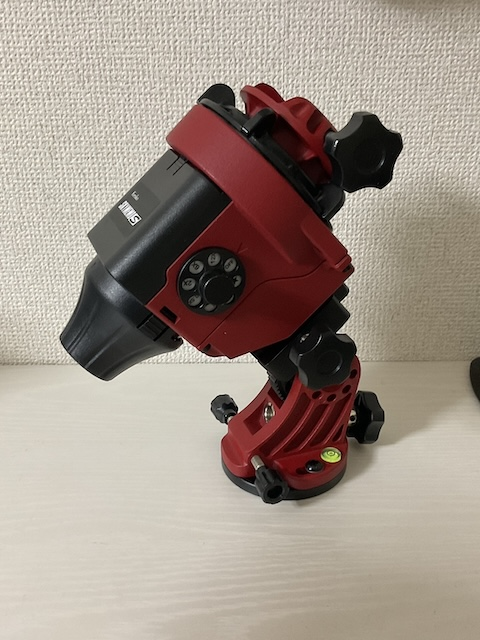
\includegraphics[width=0.8\linewidth]{sections/Kokubun/pictures/main.jpg}
    \caption{スカイメモS本体}
    \label{本体}
  \end{minipage}
  \begin{minipage}{0.45\linewidth}
    \centering
    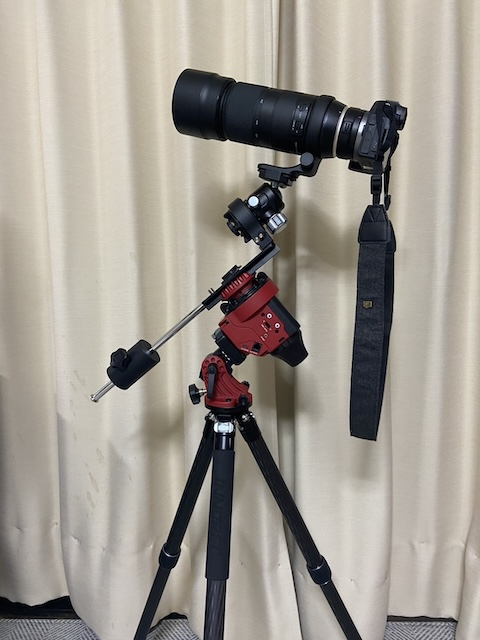
\includegraphics[width=0.8\linewidth]{sections/Kokubun/pictures/construction.jpg}
    \caption{機材構成}
    \label{構成}
  \end{minipage}
\end{figure}

\section{撮影してみた}
 8月上旬、いざ撮影です!機材自体は6月末に届きましたが、晴れそうな日と自分の予定がなかなか噛み合わず、満を持しての撮影です。はじめに、説明書の通りに月日目盛リングを回して、経度差補正目盛リングを回して\dots と頑張ってスカイメモSの極軸合わせ(正確に星を追尾するための設定)をしていくも、なかなかうまくいかず苦戦。\\
 調べてみると、リングを回してめんどうな設定をせずとも、アプリを用いれば簡単に極軸合わせができることが判明。最初に知りたかった\dots\\

気を取り直して撮影です!!福島の実家の庭先での撮影だったため、山や建物に遮られず無理なく撮れる\&導入しやすい天体が良いと思い、対象はアンドロメダ銀河にしました。まずは焦点距離\SI{100}{mm}でミラク周辺を広く撮ってアンドロメダを探し、画角の中央に持ってくることができたのち、\SI{400}{mm}までズームして撮影します。\\
 いよいよスカイメモSの性能確認です。赤道儀を用いずに星を点像として撮影するためのおおよその適正露光時間は、500ルールと呼ばれる以下の式により決まります。

\begin{equation*}
  \text{500 ÷レンズの焦点距離}=\text{適正露光時間}
\end{equation*}

今回は焦点距離が\SI{400}{mm}なので、赤道儀がない場合は1.25秒が限度となります。このスカイメモSを用いることで30秒程度露光できれば御の字だな~程度に思いながら撮影を始めます(\SI{400}{mm}で撮影を始めたつもりが、ズームリングを十分に回し切れておらず、すべて\SI{366}{mm}で撮っていたことに撮影後に気づく\dots 撮影に失敗はつきもの\dots)。\\
 まあ\SI{400}{mm}も\SI{366}{mm}もほぼ変わらないので大丈夫でしょう。まずは8秒からです。\\

\begin{figure}[H]
  \centering
  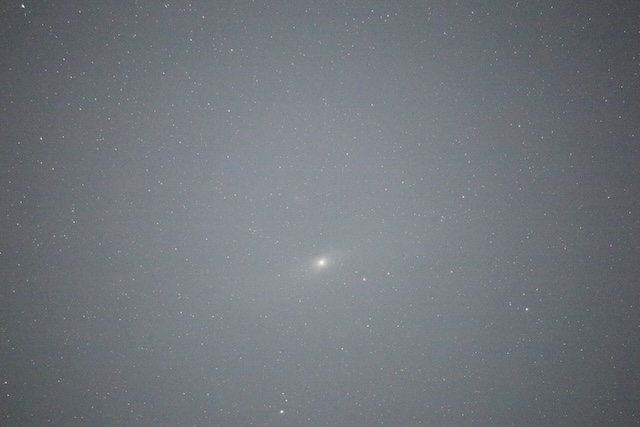
\includegraphics[width=0.7\linewidth]{sections/Kokubun/pictures/ss8.JPG}
  \caption{露光時間8秒}
  \label{ss8}
\end{figure}

\noindent
いいですね。ピントは少し甘い気がしますが、星が点で写っています。次は15秒!と思ったら15秒での撮影データがカメラにありませんでした。撮り忘れです。失敗はつきもの\dots\\

次は30秒です。

\begin{figure}[H]
  \centering
  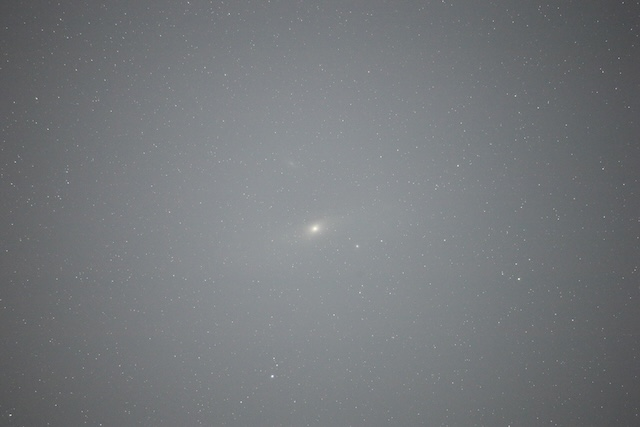
\includegraphics[width=0.7\linewidth]{sections/Kokubun/pictures/ss30.JPG}
  \caption{露光時間30秒}
  \label{ss30}
\end{figure}

\noindent
ちゃんと止まってくれています。すごい。この時点で満足ですが、一応60秒でも撮影してみましょう。

\begin{figure}[H]
  \centering
  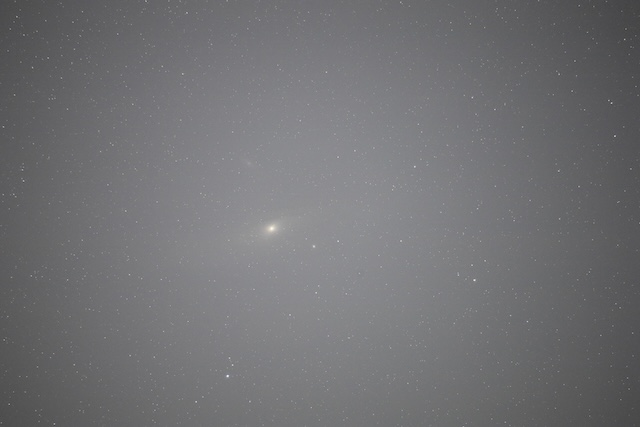
\includegraphics[width=0.7\linewidth]{sections/Kokubun/pictures/ss60.JPG}
  \caption{露光時間60秒}
  \label{ss60}
\end{figure}

\noindent
止まってる。すごすぎる。大満足です。\\

試行錯誤しながら撮影すること2時間。飽き性と寒さ(福島の夜は夏でも\SI{10}{\degreeCelsius}以下になる)と眠さから、最後に120秒で撮影して撤収することにしました。

\begin{figure}[H]
  \centering
  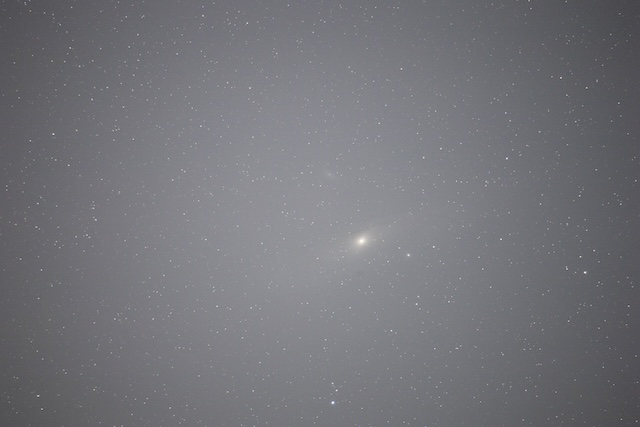
\includegraphics[width=0.7\linewidth]{sections/Kokubun/pictures/ss120.JPG}
  \caption{露光時間120秒}
  \label{ss120}
\end{figure}

\noindent
星が線になることなく完全な点として写っています。スカイメモS、ヤバい、ヤバすぎる。撮影してデータを確認するたび、感動のあまり、「うわっ、すご\dots やば\dots 」と心の声が漏れてしまいました。


\clearpage

\section{まとめ}
 今回はポータブル赤道儀「スカイメモS」のレビューでした。ポータブル赤道儀はしっかりしたガチの赤道儀より性能が劣るのではないか\dots とはじめは少し心配でしたが、杞憂に終わって安堵しました。値段が安い、性能が良い、持ち運びが楽、セッティングも楽、メンテナンスも楽、と非常に素晴らしい機材です。天体写真を撮ってみたいけどお金が\dots という方は購入を検討してみても良いかもしれません。\\
 最後に、スカイメモSを使って撮影した写真をいくつか載せて終わりにします。すべて前述のTamronのレンズで\SI{400}{mm}で撮影したものをSirilでスタック後にGIMPで調整したものになります。\\
 お読みいただきありがとうございました!!!!\\


\begin{figure}[H]
  \centering
  \begin{minipage}{0.48\linewidth}
    \centering
    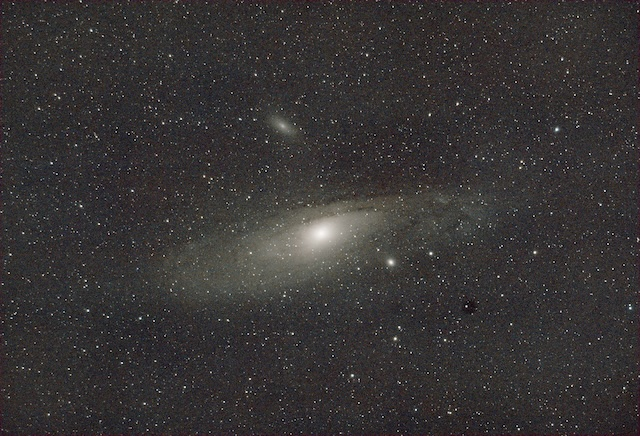
\includegraphics[width=\linewidth]{sections/Kokubun/pictures/M31.jpg}
    \caption{M31(アンドロメダ銀河)\\
    8秒×1枚+60秒×14枚+120秒×1枚}
    \label{M31}
  \end{minipage}
  \begin{minipage}{0.48\linewidth}
    \centering
    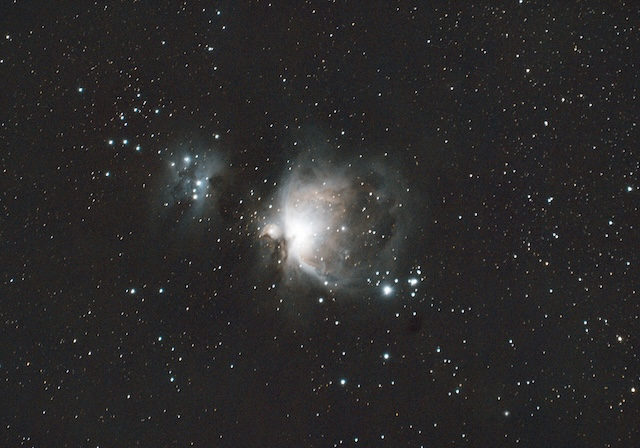
\includegraphics[width=\linewidth]{sections/Kokubun/pictures/M42.jpg}
    \caption{M42(オリオン大星雲)\\
    30秒×24枚}
    \label{M42}
  \end{minipage}
\end{figure}


\begin{figure}[H]
  \centering
  \begin{minipage}{0.48\linewidth}
    \centering
    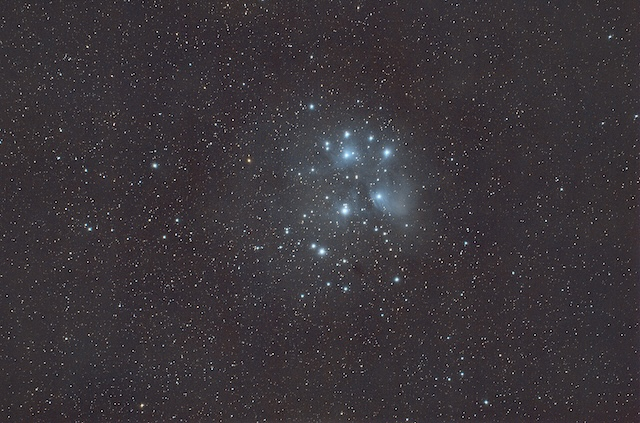
\includegraphics[width=\linewidth]{sections/Kokubun/pictures/M45.jpg}
    \caption{M45(プレアデス星団)\\
  30秒×57枚}
  \label{M45}
  \end{minipage}
  \begin{minipage}{0.48\linewidth}
    \centering
    \includegraphics[width=\linewidth]{sections/Kokubun/pictures/NGC2024_国分.jpg}
    \caption{M78、燃える樹、馬頭星雲\\
  30秒×105枚}
  \label{M4}
  \end{minipage}
\end{figure}




\end{document}
